\documentclass{beamer}
\usetheme{simple}
\usepackage[english]{babel}
\usepackage[utf8]{inputenc} 
\usepackage{lmodern}
\usepackage{ragged2e}
\usefonttheme[onlymath]{serif} 
\usepackage[scale=2]{ccicons} 
% \setbeamertemplate{caption}[numbered]
\usepackage{copyrightbox}

\usepackage{graphicx,hyperref,url,pgfplots}
\usepackage{amsmath} 
\usepackage{array,booktabs}
\usepackage{bibentry}
\usepackage[alf,abnt-etal-list=0,abnt-etal-cite=2]{abntex2cite}
\usepackage[normalem]{ulem}
\pgfplotsset{compat=1.13}  

\setbeamercovered{invisible} 
% \newcommand{\pausar}{\pause}
\newcommand{\pausar}{\pause}
\newcommand{\df}[1]{\,\mathrm{d}#1}
\newcommand{\parcial}[3]{\dfrac{\partial^{#1}#2}{\partial #3^{#1}}}
\newcommand{\cpright}[2]{\copyrightbox[b]{#1}{\tiny Source: #2}}

\usepackage{tikz}
\usetikzlibrary{automata,positioning}
\usepackage{xcolor}
\usetikzlibrary{scopes}
\usepackage{verbatim}
\usetikzlibrary{patterns}


\usepackage{listings}
	\definecolor{codegreen}{rgb}{0,0.6,0}
	\definecolor{codegray}{rgb}{0.5,0.5,0.5}
	\definecolor{codepurple}{rgb}{0.58,0,0.82}
	\definecolor{backcolour}{rgb}{0.92,0.92,0.92}
	\lstset{language=Python, 
	backgroundcolor=\color{backcolour},   
	commentstyle=\color{codegreen},
	keywordstyle=\color{magenta},
	numberstyle=\tiny\color{codegray},
	stringstyle=\color{codepurple},
	basicstyle=\fontsize{8}{11}\ttfamily,
	frame=lines,
%	numbers=left,
	tabsize=2,
	morekeywords={models, lambda, forms}}


% --------------------------------------------------------------------------------------------

\title{Mobile Robots}
\subtitle{ROS - Robot Operating System}
\date{\today}
\author[Jeferson José de Lima]{
  \textbf{Professor}: Jeferson José de Lima}
\institute{Academic Department of Informatics (DAINF) \\ Federal University of Technology - Paraná (UTFPR) at Pato Branco, PR, Brazil}

\begin{document}
\maketitle
\justify


\begin{frame}{Useful Information}
	\begin{block}{links:}
		\begin{enumerate}
			\item \href{https://moodle.utfpr.edu.br/course/view.php?id=14218}{Moodle}
			\item \href{https://gitlab.com/cursoseaulas/robotica-movel/-/wikis/home}{Mobile Robots - Gitlab Page}
			\item \href{http://www.rsl.ethz.ch/education-students/lectures/ros.html}{ETH Programming for Robotics - ROS}
		\end{enumerate}
	\end{block}
\end{frame}



\begin{frame}{What is ROS?}
	\framesubtitle{ROS - Robot Operating System}
	\centering
	
\includegraphics[width=0.4\textwidth]{./images/roslogo.png}
	\begin{block}{About ROS}
		The Robot Operating System (ROS) is a flexible framework for writing robot software. It is a collection of tools, libraries, and conventions that aim to simplify the task of creating complex and robust robot behavior across a wide variety of robotic platforms.

		{\tiny \textbf{More info}: 
		https://www.ros.org/about-ros/}
	\end{block}
\end{frame}


\begin{frame}{History of ROS}
	\framesubtitle{}
	\begin{itemize}
		\item Originally developed in 2007 at the Stanford Artificial Intelligence Laboratory;
		\item Since 2013 managed by Open Source Robotics Foundation, Inc. (OSRF);
		\item Today used by many robots, universities and companies\footnote[frame]{\textcolor{purple}{ https://rosindustrial.org/about/description }};
		\item De facto standard for robot programming;
	\end{itemize}
\end{frame}


\begin{frame}{ROS Philosophy}
	\framesubtitle{}
	\begin{itemize}
		
		\item \textbf{Peer to peer}: Individual programs communicate over defined API (ROS messages, services, etc.).
		\item \textbf{Distributed}: Programs can be run on multiple computers and communicate over the network.
		\item \textbf{Multi-lingual}: ROS modules can be written in any language for which a client library exists (C++, Python, MATLAB, Java, etc.).
		\item \textbf{Light-weight}: Stand-alone libraries are wrapped around with a thin ROS layer.
		\item \textbf{Free and open-source}: Most ROS software is open-source and free to use.

	\end{itemize}
\end{frame}

\begin{frame}[fragile]{ROS Master}
	\framesubtitle{ }
	\begin{minipage}{0.47\textwidth}
    \begin{itemize}
        \item Manages the communication between nodes (processes)
        \item Every node registers at startup with the master
    \end{itemize}
	
	\vspace{0.3in}

	\begin{itemize}
		\item Start a master with:

		\begin{lstlisting}
			$ roscore
		\end{lstlisting}

		\item \textbf{roscore} will start up a ROS Master, a ROS Parameter Server and a rosout logging node
		\end{itemize}

	

\end{minipage}
\begin{minipage}{0.5\textwidth}
	\centering
\resizebox{0.85\textwidth}{!}{
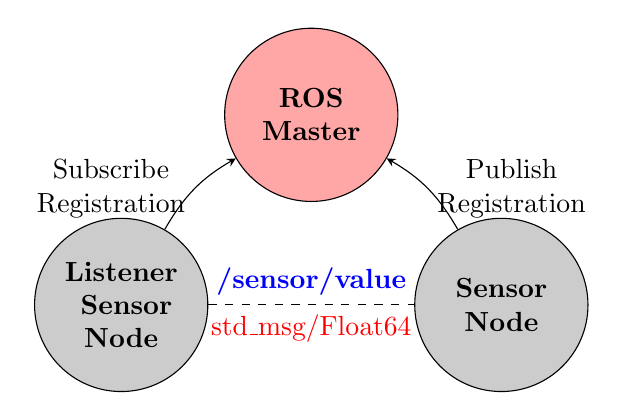
\begin{tikzpicture}[>=stealth,
    auto,
    state/.append style={fill=black!20, circle, draw, minimum size=2.2cm},
    node distance=1.2cm,
    every text node part/.style={align=center}] 
    \node[state, fill=red!35] (MASTER) {\textbf{ROS} \\ \textbf{Master}};
    \node[state,below right=of MASTER] (SENSOR) {\textbf{Sensor} \\ \textbf{Node}};
    \node[state,below left=of MASTER] (LISTENER) {\textbf{Listener} \\ \textbf{ Sensor} \\ \textbf{Node}};
    \draw (LISTENER) edge[->,bend left=15] node[left] {Subscribe \\ Registration} (MASTER);
    \draw (SENSOR) edge[->,bend right=15] node[right] {Publish \\ Registration} (MASTER);
    \draw (LISTENER) edge[-, dashed] node[blue] {\textbf{/sensor/value}} node[below, red] {std\_msg/Float64} (SENSOR);

\end{tikzpicture}}

\end{minipage}
\end{frame}


\begin{frame}[fragile]{ROS Nodes}
	\framesubtitle{ }
	\begin{minipage}{0.47\textwidth}
    \begin{itemize}
        \item First item
        \item Second item
        \item Third item
    \end{itemize}
	\begin{lstlisting}
		$ roscore
    \end{lstlisting}
\end{minipage}
\begin{minipage}{0.5\textwidth}
	\centering
\resizebox{0.85\textwidth}{!}{
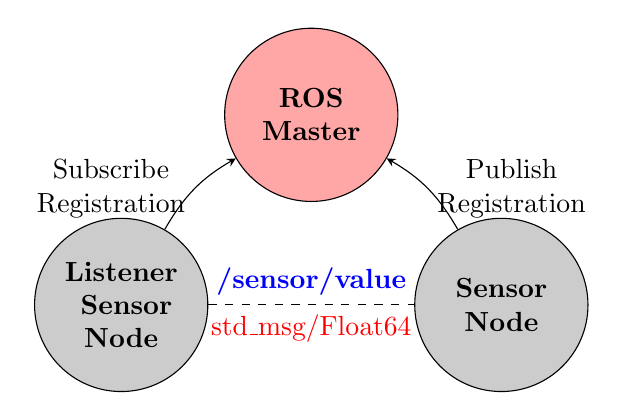
\begin{tikzpicture}[>=stealth,
    auto,
    state/.append style={fill=black!20, circle, draw, minimum size=2.2cm},
    node distance=1.2cm,
    every text node part/.style={align=center}] 
    \node[state, fill=red!35] (MASTER) {\textbf{ROS} \\ \textbf{Master}};
    \node[state,below right=of MASTER] (SENSOR) {\textbf{Sensor} \\ \textbf{Node}};
    \node[state,below left=of MASTER] (LISTENER) {\textbf{Listener} \\ \textbf{ Sensor} \\ \textbf{Node}};
    \draw (LISTENER) edge[->,bend left=15] node[left] {Subscribe \\ Registration} (MASTER);
    \draw (SENSOR) edge[->,bend right=15] node[right] {Publish \\ Registration} (MASTER);
    \draw (LISTENER) edge[-, dashed] node[blue] {\textbf{/sensor/value}} node[below, red] {std\_msg/Float64} (SENSOR);

\end{tikzpicture}}

\end{minipage}
\end{frame}



\begin{frame}[fragile]{ROS Topics}
	\framesubtitle{ }
	\begin{minipage}{0.47\textwidth}
    \begin{itemize}
        \item First item
        \item Second item
        \item Third item
    \end{itemize}
	\begin{lstlisting}
		$ roscore
    \end{lstlisting}
\end{minipage}
\begin{minipage}{0.5\textwidth}
	\centering
\resizebox{0.85\textwidth}{!}{
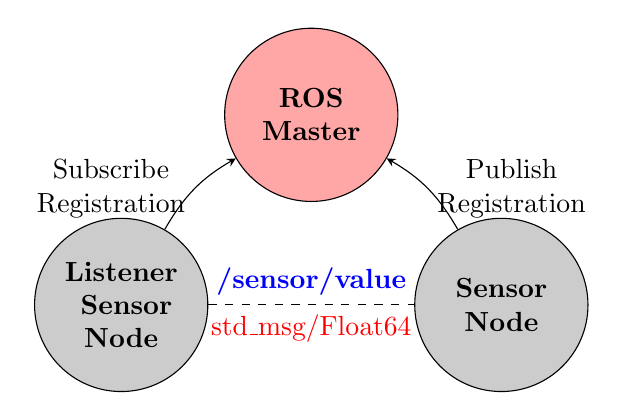
\begin{tikzpicture}[>=stealth,
    auto,
    state/.append style={fill=black!20, circle, draw, minimum size=2.2cm},
    node distance=1.2cm,
    every text node part/.style={align=center}] 
    \node[state, fill=red!35] (MASTER) {\textbf{ROS} \\ \textbf{Master}};
    \node[state,below right=of MASTER] (SENSOR) {\textbf{Sensor} \\ \textbf{Node}};
    \node[state,below left=of MASTER] (LISTENER) {\textbf{Listener} \\ \textbf{ Sensor} \\ \textbf{Node}};
    \draw (LISTENER) edge[->,bend left=15] node[left] {Subscribe \\ Registration} (MASTER);
    \draw (SENSOR) edge[->,bend right=15] node[right] {Publish \\ Registration} (MASTER);
    \draw (LISTENER) edge[-, dashed] node[blue] {\textbf{/sensor/value}} node[below, red] {std\_msg/Float64} (SENSOR);

\end{tikzpicture}}

\end{minipage}
\end{frame}



\begin{frame}[fragile]{ROS Messages}
	\framesubtitle{ }
	\begin{minipage}{0.47\textwidth}
    \begin{itemize}
        \item First item
        \item Second item
        \item Third item
    \end{itemize}
	\begin{lstlisting}
		$ roscore
    \end{lstlisting}
\end{minipage}
\begin{minipage}{0.5\textwidth}
	\centering
\resizebox{0.85\textwidth}{!}{
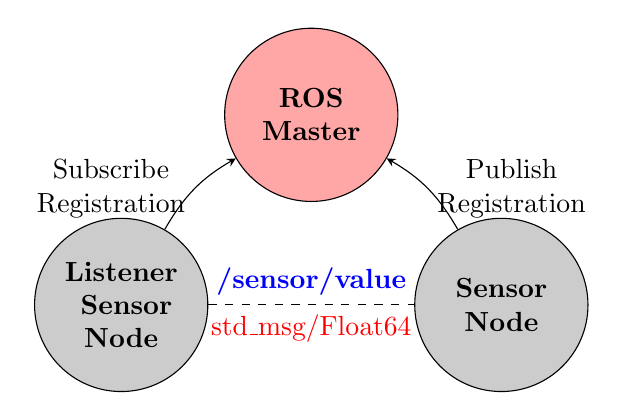
\begin{tikzpicture}[>=stealth,
    auto,
    state/.append style={fill=black!20, circle, draw, minimum size=2.2cm},
    node distance=1.2cm,
    every text node part/.style={align=center}] 
    \node[state, fill=red!35] (MASTER) {\textbf{ROS} \\ \textbf{Master}};
    \node[state,below right=of MASTER] (SENSOR) {\textbf{Sensor} \\ \textbf{Node}};
    \node[state,below left=of MASTER] (LISTENER) {\textbf{Listener} \\ \textbf{ Sensor} \\ \textbf{Node}};
    \draw (LISTENER) edge[->,bend left=15] node[left] {Subscribe \\ Registration} (MASTER);
    \draw (SENSOR) edge[->,bend right=15] node[right] {Publish \\ Registration} (MASTER);
    \draw (LISTENER) edge[-, dashed] node[blue] {\textbf{/sensor/value}} node[below, red] {std\_msg/Float64} (SENSOR);

\end{tikzpicture}}

\end{minipage}
\end{frame}



\begin{frame}[t, allowframebreaks]
	\frametitle{Referências}
	\bibliography{../references.bib}
\end{frame}

\end{document}

